% SWOT Rain EGU 2026 Poster — 250 m/px CNN version only
% A0 landscape, CLS corporate branding
% Compile with: make pdf (uses tectonic)

\documentclass[final]{beamer}
\graphicspath{{images/}}
\usepackage[orientation=landscape, size=a0, scale=1.1]{beamerposter}

% ---------------------------------------------------------------------------
% Page geometry
% ---------------------------------------------------------------------------
\usepackage{geometry}
\geometry{
    top=0mm,
    bottom=10mm,
    left=15mm,
    right=15mm
}

% ---------------------------------------------------------------------------
% Packages
% ---------------------------------------------------------------------------
\usepackage[utf8]{inputenc}
\usepackage{amsmath}
\usepackage{amsfonts}
\usepackage{amssymb}
\usepackage{graphicx}
\usepackage{booktabs}
\usepackage{ragged2e}
\usepackage{hyperref}
\usepackage{multicol}

% ---------------------------------------------------------------------------
% CLS Poster Theme (landscape mode)
% ---------------------------------------------------------------------------
\usepackage[landscape]{clsposter}

\hypersetup{colorlinks=true, urlcolor=CLSBlue, linkcolor=CLSBlue, citecolor=CLSBlue}

% ---------------------------------------------------------------------------
% Compact spacing
% ---------------------------------------------------------------------------
\setlength{\parskip}{0pt}
\setbeamersize{text margin left=0.8cm, text margin right=0.8cm}
\setbeamerfont{caption}{size=\footnotesize}
\setlength{\abovecaptionskip}{1pt}
\setlength{\belowcaptionskip}{0pt}

% Tighter block padding
\makeatletter
\renewenvironment{clsblock}[1]{%
  \begin{center}
  \begin{tikzpicture}
  \node[
    draw=CLSBlue, line width=2pt,
    fill=CLSLightGray,
    rounded corners=5mm,
    inner sep=8pt
  ] (blockbox) \bgroup
    \begin{minipage}{0.93\linewidth}
      \vspace{0.15cm}
      {\centering\LARGE\bfseries\textcolor{CLSBlue}{#1}\par}
      \vspace{0.2cm}
      \justifying
}{%
      \vspace{0.15cm}
    \end{minipage}
  \egroup;
  \draw[left color=CLSGradientBlue, right color=CLSGradientGreen, line width=3pt]
    ([yshift=0pt]blockbox.north west) -- ([yshift=0pt]blockbox.north east);
  \end{tikzpicture}
  \end{center}
}
\renewenvironment{clshighlight}[1]{%
  \begin{center}
  \begin{tikzpicture}
  \node[
    draw=CLSTeal, line width=2pt,
    fill=CLSTeal!10,
    rounded corners=5mm,
    inner sep=8pt
  ] (blockbox) \bgroup
    \begin{minipage}{0.93\linewidth}
      \vspace{0.15cm}
      {\centering\LARGE\bfseries\textcolor{CLSTeal}{#1}\par}
      \vspace{0.2cm}
      \justifying
}{%
      \vspace{0.15cm}
    \end{minipage}
  \egroup;
  \draw[CLSTeal, line width=3pt]
    (blockbox.north west) -- (blockbox.north east);
  \end{tikzpicture}
  \end{center}
}
\makeatother

% ===========================================================================
% Poster metadata
% ===========================================================================

\postertitle{%
  Precipitation Detection in Open Ocean with SWOT%
  \\ at Sub-Kilometer Resolution%
}

\posterauthor{%
  Aur\'elien Colin\textsuperscript{1},
  Romain Husson\textsuperscript{1},
  Bruno Picard\textsuperscript{2}%
}

\posterinstitute{%
  \textsuperscript{1} Collecte Localisation Satellites (CLS),
  Plouzan\'e, France \quad
  \textsuperscript{2} Fluctus SAS, Rabastens, France%
}

\posterconference{EGU General Assembly 2026}
\posterdate{27 April -- 2 May 2026, Vienna, Austria}

\posterlogos{%
  \hspace{1.5cm}
\includegraphics[height=4cm]{images/cnes_logo.png}%
  \hspace{1.5cm}
\includegraphics[height=4cm]{images/fluctus_logo.png}%
}

% ===========================================================================
\begin{document}
\begin{frame}{}

\maketitle
\vspace{-0.5cm}

% ===================== ROW 1 =====================
\begin{columns}[T]

  % --- Col 1: Introduction ---
  \begin{column}{0.32\linewidth}
    \begin{clsblock}{Introduction}
      Precipitation is a fundamental component of the hydrological cycle,
      yet rain rate estimation over the open ocean remains a challenge.
      Ground-based radars such as NEXRAD~[1] provide high-resolution
      measurements but are limited to coastal areas. Satellite products
      like IMERG~[2] offer global coverage at $\sim$8~km resolution, too
      coarse for fine-scale studies.

      \vspace{0.15cm}
      The Surface Water and Ocean Topography (SWOT) mission~[3] carries
      the Ka-band Radar Interferometer (KaRIn), a SAR operating at
      35.75~GHz. Originally designed for altimetry, KaRIn is sensitive to
      atmospheric hydrometeors at \textbf{250~m/pixel}---matching NEXRAD
      resolution in range---and provides continuous data over both coastal
      zones and open ocean.

      \vspace{0.15cm}
      We present a machine learning framework to estimate precipitation
      rates from SWOT 250~m observations, trained against NEXRAD
      collocations and validated with independent IMERG time series.
    \end{clsblock}
  \end{column}

  % --- Col 2: Data & Methods ---
  \begin{column}{0.34\linewidth}
    \begin{clsblock}{Data \& Methods}
      \textbf{Training dataset.}
      A NEXRAD/SWOT collocation dataset of \textbf{7\,009 patches}
      (512$\times$512~px at 250~m/pixel) was built between August 2023 and
      February 2025. Among these, 1\,090 patches contain precipitation
      ($>$1~mm/h on $>$1\% of pixels). Collocations are restricted to
      $<$3~min temporal offset and $<$170~km range from a WSR-88D station.

      \vspace{0.15cm}
      \textbf{Model architecture.}
      A U-Net (depth=4, Swish activation, BatchNorm) takes four input
      channels: incidence-corrected $\sigma_0$ (dB), total coherence,
      incidence angle, and model wind speed (projected from the 2~km
      product). The output is a pixel-wise precipitation rate (mm/h).

      \vspace{0.15cm}
      \textbf{Training strategy.}
      The loss combines regression MAE (99\%) and categorical MAE (1\%).
      Pixel weights decay linearly with distance to the nearest NEXRAD
      station (1 at 0~km, 0 at 225~km); null-DPR pixels are
      down-weighted to 0.1\%. Quantile mapping aligns the output
      distribution with NEXRAD statistics.

      \vspace{0.15cm}
      \textbf{Ensemble.}
      Five independently trained models produce a consensus score based on
      inter-model agreement, providing a proxy for prediction confidence.
    \end{clsblock}
  \end{column}

  % --- Col 3: 250 m inference example ---
  \begin{column}{0.32\linewidth}
    \begin{clshighlight}{Inference at 250~m/pixel}
      \centering
      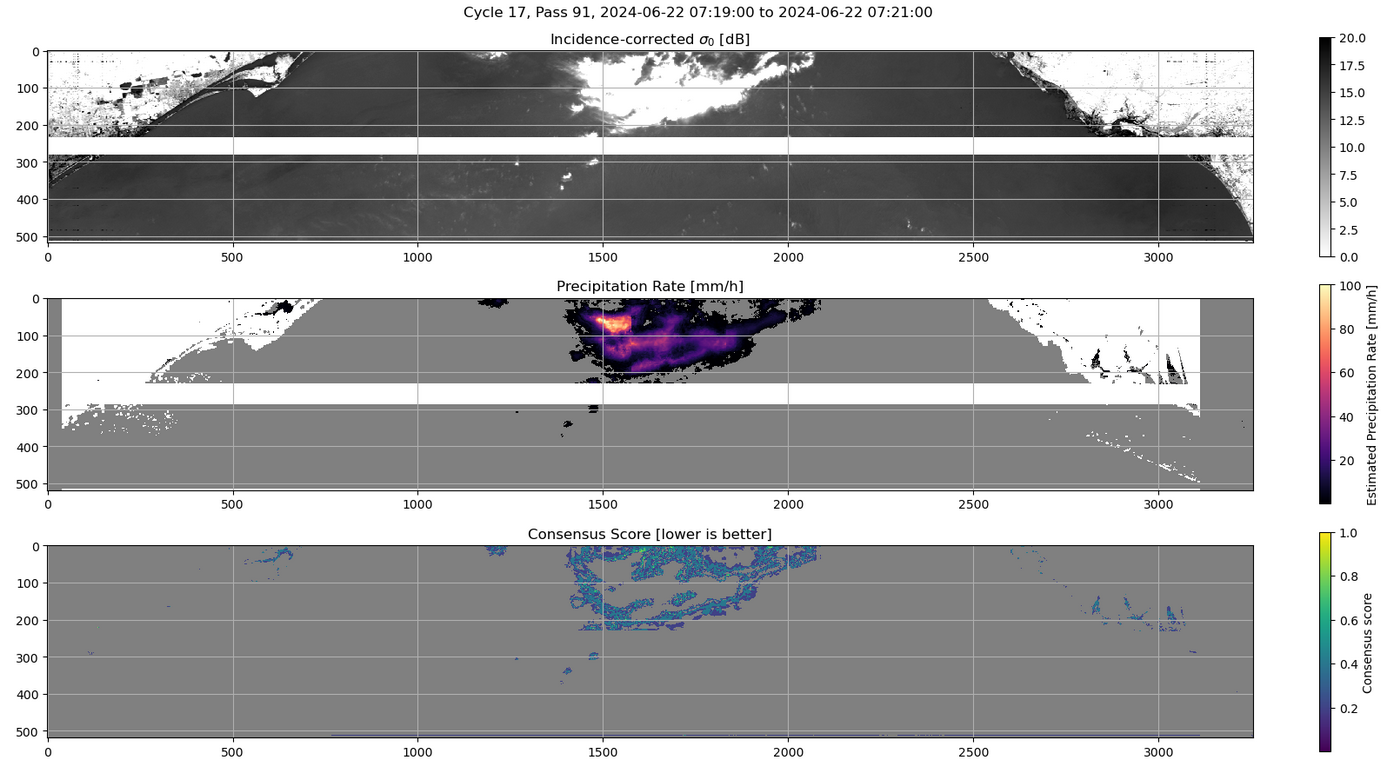
\includegraphics[width=0.92\linewidth]{images/inference_250m.png}

      \vspace{0.15cm}
      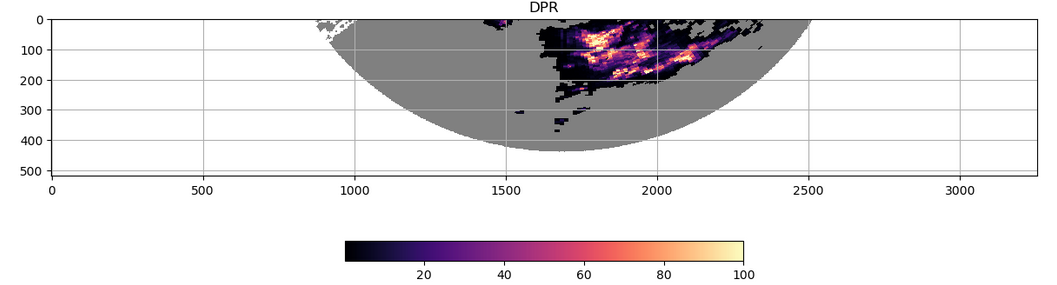
\includegraphics[width=0.92\linewidth]{images/inference_dpr_250m.png}

      \vspace{0.15cm}
      \small Cycle 17, Pass 81 (June 2024). \textbf{Top:} SWOT
      $\sigma_0$ (left swath) and ensemble mean precipitation rate (mm/h)
      with consensus score (lower is better). \textbf{Bottom:} Collocated
      NEXRAD Digital Precipitation Rate for validation.
    \end{clshighlight}
  \end{column}

\end{columns}

\vspace{0.1cm}

% ===================== ROW 2 =====================
\begin{columns}[T]

  % --- Col 1: Evaluation against NEXRAD ---
  \begin{column}{0.32\linewidth}
    \begin{clsblock}{Evaluation against NEXRAD}
      \textbf{Categorical accuracy} is evaluated on three precipitation
      classes: [0--1), [1--10), and $\geq$10~mm/h. The ensemble reaches
      \textbf{68.4\%} accuracy, a marginal improvement over individual
      models (63.6--68.0\%).

      \vspace{0.15cm}

      \centering
      \begin{table}
        \small
        \begin{tabular}{l@{\hspace{0.6cm}}ccc}
          \toprule
          & \multicolumn{3}{c}{\textbf{Predicted (mm/h)}} \\
          \cmidrule(lr){2-4}
          \textbf{NEXRAD} & {[0--1)} & {[1--10)} & {$\geq$10} \\
          \midrule
          {[0--1) mm/h}   & \textbf{94.1\%} & 20.9\%          & 11.2\% \\
          {[1--10) mm/h}  & 5.3\%           & \textbf{45.7\%} & 23.5\% \\
          {$\geq$10 mm/h} & 0.5\%           & 33.4\%          & \textbf{65.4\%} \\
          \bottomrule
        \end{tabular}
        \caption{Ensemble confusion matrix (column-normalized).}
      \end{table}

      \justifying
      \small
      The model accurately identifies rain-free areas (94.1\%).
      Heavy rainfall ($\geq$10~mm/h) is detected with 65.4\% accuracy.
      Moderate rainfall ([1--10)~mm/h) is the hardest class,
      with 33.4\% misclassified as heavy rain.
    \end{clsblock}
  \end{column}

  % --- Col 2: IMERG validation + Mollweide ---
  \begin{column}{0.34\linewidth}
    \begin{clsblock}{Global Validation against IMERG}
      \begin{columns}[T]
        \begin{column}{0.48\linewidth}
          \centering
          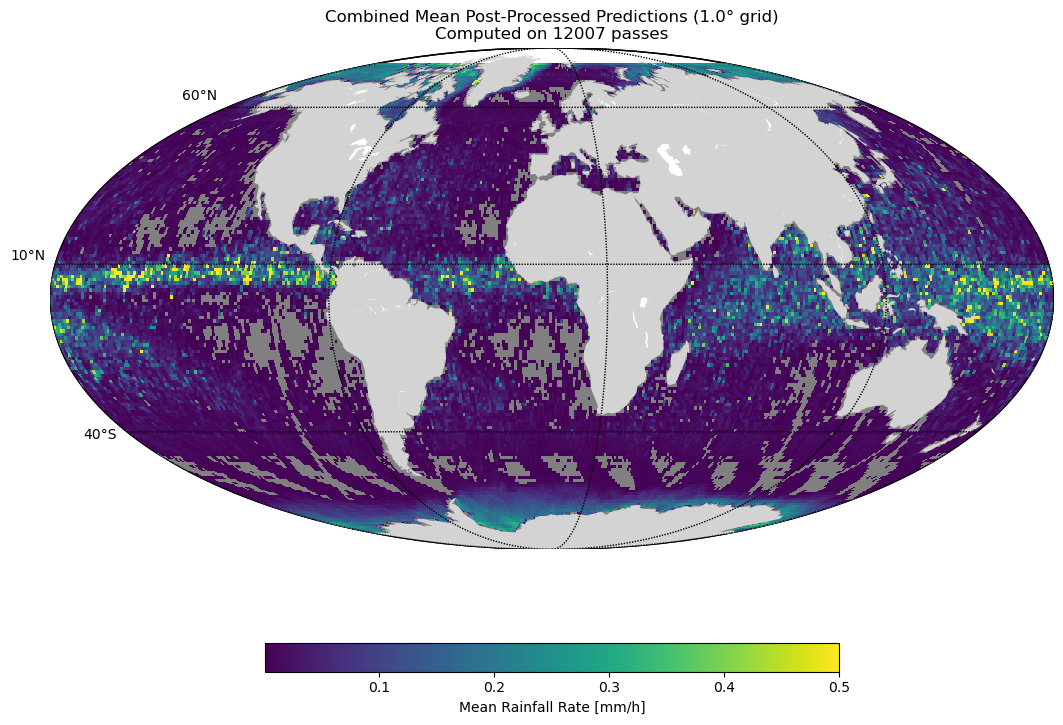
\includegraphics[width=\linewidth]{images/mollweide_mean_rainfall.png}
        \end{column}
        \begin{column}{0.48\linewidth}
          \centering
          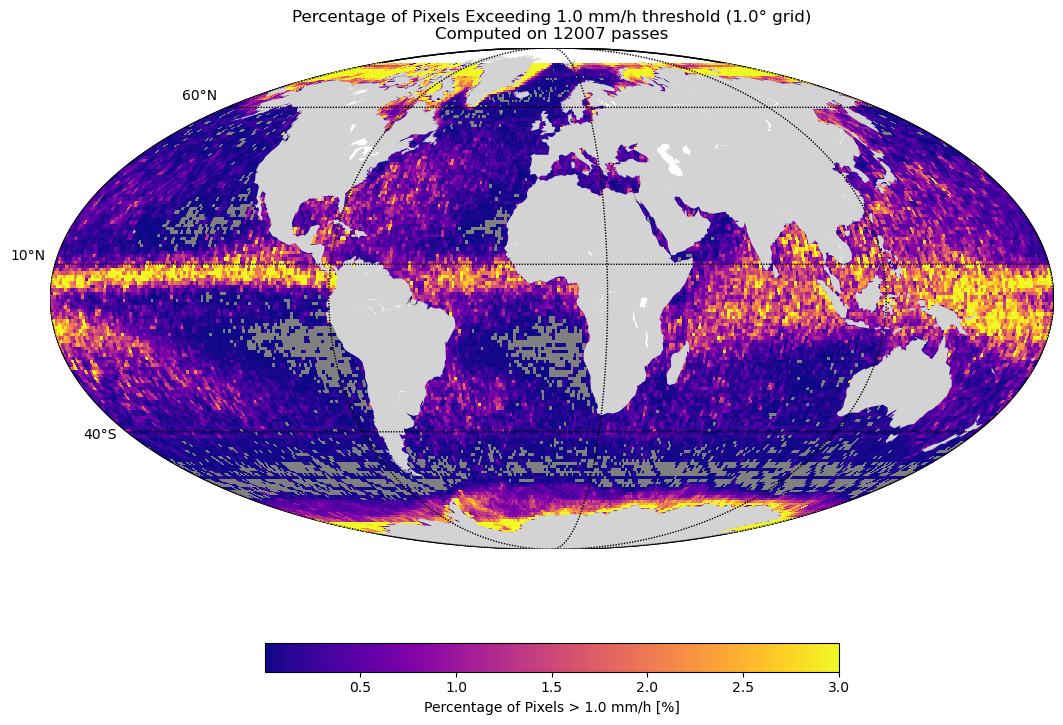
\includegraphics[width=\linewidth]{images/mollweide_pct_above_1mmh.png}
        \end{column}
      \end{columns}
      \small Mean rainfall rate (left) and percentage of pixels
      $>$1~mm/h (right) on a 1.0$^\circ$ grid (12\,007 passes).
      The ITCZ is clearly delineated; spatial patterns match
      IMERG climatology.

      \vspace{0.1cm}

      \begin{columns}[T]
        \begin{column}{0.32\linewidth}
          \centering
          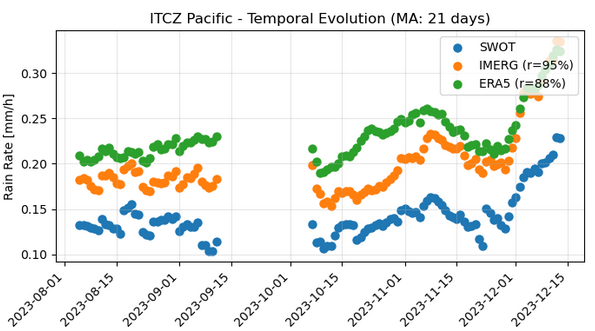
\includegraphics[width=\linewidth]{images/timeseries_itcz_pacific.png}

          \small Pacific ITCZ\\ \textbf{r\,=\,95\%}
        \end{column}
        \begin{column}{0.32\linewidth}
          \centering
          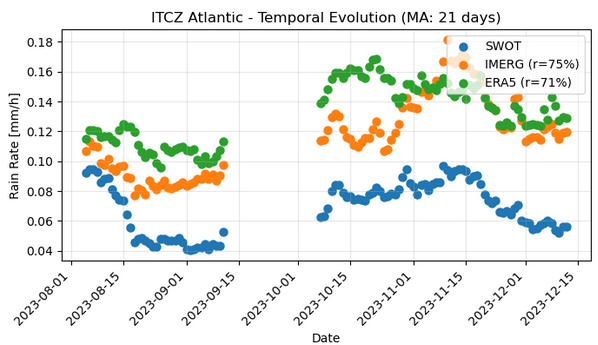
\includegraphics[width=\linewidth]{images/timeseries_itcz_atlantic.png}

          \small Atlantic ITCZ\\ \textbf{r\,=\,75\%}
        \end{column}
        \begin{column}{0.32\linewidth}
          \centering
          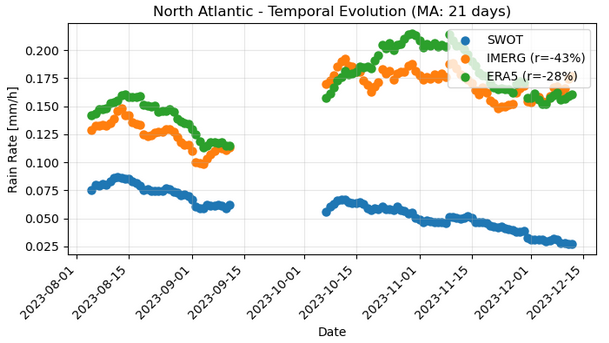
\includegraphics[width=\linewidth]{images/timeseries_north_atlantic.png}

          \small North Atlantic\\ \textbf{r\,=\,$-$43\%}
        \end{column}
      \end{columns}
      \vspace{0.05cm}
      \small 21-day moving average vs.\ IMERG and ERA5. High
      correlation in the tropics; sharp degradation in the North
      Atlantic where stratiform precipitation dominates.
    \end{clsblock}
  \end{column}

  % --- Col 3: Conclusions + Refs ---
  \begin{column}{0.32\linewidth}
    \begin{clsblock}{Conclusions \& Perspectives}
      \begin{itemize}\setlength{\itemsep}{4pt}
        \item SWOT KaRIn observations at 250~m/pixel can be exploited to
              estimate precipitation rates over the open ocean, where no
              ground-based radar coverage exists.

        \item The U-Net ensemble achieves \textbf{68\%} categorical
              accuracy against NEXRAD, comparable to the consistency
              between two independent NEXRAD stations~[1].

        \item Temporal correlation with IMERG reaches \textbf{95\%} in
              the Pacific ITCZ and \textbf{75\%} in the Atlantic ITCZ,
              demonstrating skill in tropical convective regimes.

        \item \textbf{Open question:} performance degrades at
              mid-latitudes (North Atlantic: r\,=\,$-$43\%), suggesting
              reduced sensitivity to stratiform precipitation. Further
              investigation is needed to characterize this limitation.

        \item \textbf{Perspectives:} these results are consistent with
              C-band SAR rainfall retrievals from the Sentinel-1
              constellation~[4]. Integration into the standard SWOT
              unsmoothed product is under discussion, which would unlock
              precipitation data in data-sparse oceanic regions.
      \end{itemize}
    \end{clsblock}

    \vspace{0.15cm}

    \begin{clsblock}{References}
      \footnotesize
      [1]~T.~D.~Crum, R.~L.~Alberty,
      \textit{Bull.~Am.~Meteorol.~Soc.}, 74(9), 1993.\\[2pt]
      {[2]}~G.~J.~Huffman \textit{et al.},
      NASA GPM IMERG ATBD v06, 2019.\\[2pt]
      {[3]}~R.~Morrow \textit{et al.},
      \textit{Front.~Mar.~Sci.}, 6:232, 2019.\\[2pt]
      {[4]}~A.~Mouche \textit{et al.},
      \textit{Proc.~IGARSS}, 2017.

      \vspace{0.2cm}
      \textbf{Acknowledgements.}
      This work was supported by CNES.
      SWOT data: NASA/CNES. NEXRAD data: NOAA.
      IMERG data: NASA GES DISC.
    \end{clsblock}
  \end{column}

\end{columns}

\posterfooter

\end{frame}
\end{document}
